\documentclass[conference]{IEEEtran}
%\documentclass[sigconf]{acmart}
\makeatletter
\def\ps@headings{%
\def\@oddhead{\mbox{}\scriptsize\rightmark \hfil \thepage}%
\def\@evenhead{\scriptsize\thepage \hfil \leftmark\mbox{}}%
\def\@oddfoot{}%
\def\@evenfoot{}}
\makeatother
\pagestyle{empty}
\usepackage{url}
\usepackage{graphicx,subfigure}
\usepackage{epstopdf}
\usepackage{amsmath}
\usepackage{algorithm}
\usepackage{algpseudocode}
\usepackage{amsmath}
\usepackage{amssymb}
\usepackage{amsthm}
\usepackage{epsfig}
\newtheorem{theorem}{Theorem}
\renewcommand{\algorithmicrequire}{\textbf{Input:}} % Use Input in the format of Algorithm
\renewcommand{\algorithmicensure}{\textbf{Output:}} % Use Output in the format of Algorithm
\usepackage{amsfonts}
%\newtheorem{theorem}{Theorem}[section]
\newtheorem{mydef}{Definition}[section]
%\newtheorem{lemma}{Lemma}[section]
\usepackage{multirow}
\usepackage{color}
\usepackage{array}
\usepackage{listings}
\usepackage{hyperref}
\usepackage[underline=true]{pgf-umlsd}
\newcommand{\tabincell}[2]
{\begin{tabular}
		{@{}#1@{}}#2\end{tabular}}
\usepackage{setspace}
\renewcommand{\labelitemi}{$\vcenter{\hbox{\tiny$\bullet$}}$}


\hyphenation{op-tical net-works semi-conduc-tor}




\begin{document}



\title{Predicting COVID-19 Data Trends}

\author{\IEEEauthorblockN{Caitlin Carfano}
\IEEEauthorblockA{\textit{Department of ECE Engineering} \\
\textit{Stevens Institute of Technology}\\
Hoboken, NJ \\
ccarfano@stevens.edu}
\and
\IEEEauthorblockN{Michael Takrama}
\IEEEauthorblockA{\textit{Department of ECE Engineering} \\
\textit{Stevens Institute of Technology}\\
Hoboken, NJ \\
mtakrama@stevens.edu}
\and
\IEEEauthorblockN{Calvin Weaver}
\IEEEauthorblockA{\textit{Department of ECE Engineering} \\
\textit{Stevens Institute of Technology}\\
Hoboken, NJ \\
cweaver1@stevens.edu}
}

\maketitle


\begin{abstract}
As the COVID-19 pandemic continues to impact the daily lives of everyone around the world, it has become apparent the importance of predicting trends related to the COVID-19 virus. To visualize the efficacy of vaccines, we will use artificial neural networks to predict the number of cases and deaths that will occur within the next 3 months in the USA. The obtained results could potentially provide insight into the importance of herd immunity. 
\end{abstract}

\section{Introduction}
The COVID-19 pandemic has been affecting the lives of everyone in the world. Scientists and politicians have been looking at historic data of the disease to try and predict the future path of the pandemic. With vaccines becoming more widely available, the data for COVID-19 trends becomes more interesting to study the effectiveness of high versus low vaccination rates. In this project, we will utilize training data provided by the CDC, looking at historic COVID-19 daily case numbers, number of deaths, and vaccination rates in the USA. With this data, we will predict the future case numbers and deaths while taking into account vaccination rates. Subsequently, we can determine the effect of vaccination rates on case numbers and deaths and show the importance of herd immunity. 

From the CDC's government website, we downloaded data showcasing the daily cases of COVID-19 in the USA, daily deaths caused by COVID-19 in the USA, and COVID-19 vaccine doses administered daily in the USA. These datasets have been parsed and labeled accordingly. To start, the inputs we used were daily new cases and 7-day moving average from Alabama in the past 40 day period. Utilizing both the daily new cases to train data and comparing that to the trained data from the 7-day moving average, the 7-day moving average predicted the outcome more accurately. This accuracy could be improved by feeding more training data from other states and longer periods of time, as well as adjusting the number of hidden layers and hidden layer units. 

The machine learning algorithm used in this project is the artificial neural network. It is used because it has a good fault tolerance, the ability to work with insufficient knowledge, and can dynamically grow. To implement this functionality, we will be using the sklearn.neural\_network.MLPClassifier which utilizes a multi-layer perceptron classifier [1]. The number of hidden layers and hidden layer units can be adjusted based on training data and overfitting analysis. Comparing the model versus the training data error, the accuracy score is 94.2 percent. When comparing the model versus the test data error, the accuracy score is 0.0 percent, however this is because it is highly unlikely that the model will be able to guess the precise number of new cases that will arise on any given day. The trend data is just too noisy to be matched by our model with high precision (for example if the model guessed 3001 new cases and we expected 3000, this is still extremely accurate), so instead we need to adjust how we measure the performance of our model. Such a metric would likely include the per-day error in estimated new case numbers (we can develop this measurement technique as we continue the project).

The solutions chosen for this problem are optimal because the artificial neural network has parameters that can be adjusted to optimize the predicted results based on the current dataset. The relatively low complexity and low computing power needed to achieve the results of this algorithm is important based on the resources given to complete this project [2]. This algorithm was chosen because of the pervasiveness and usefulness of artificial neural networks in various other machine learning problems. Additionally, these networks can be trained given an abundance of data, which we have access to from the CDC's website, and we can adjust the parameters accordingly. 

\section{Related Work}
Existing solutions use algorithms such as the random forest classifier and extra tree classifier (ETC) according to data from the journal article, "Forecast and prediction of COVID-19 using machine learning" [3]. The pros of the random forest classifier include lower risk of overfitting, robust to outliers, and can handle large datasets. The cons are slow training and can be potentially biased [2]. The pros and cons of the ETC are similar, but it is much faster than the random forest classifier. Additionally, data from the journal article, "A machine learning based exploration of COVID-19 mortality risk" cite using algorithms such as support vector machine models using invasive, non-invasive, and both groups [4]. The pros of the support vector machines is that they are effective for high dimensionality, but the cons are that it could be slow when given large training datasets [2].

\section{Our Solution}
Our solution to predict COVID-19 data is to use artificial neural networks.

\subsection{Description of Dataset}
For our early approach to the problem, we used a single trend graph for Alabama provided by the CDC's website. The graph contains roughly one year of daily new case numbers, as well as the 7-day new case averages from any given day. We converted string-format dates into raw integer Unix timestamps in order to make plotting the data easier. We also preprocessed the input data using the sklearn.preprocessing.StandardScaler [5] in order to normalize the input data for easier interpretation by the network.

\begin{figure}
    \centering
    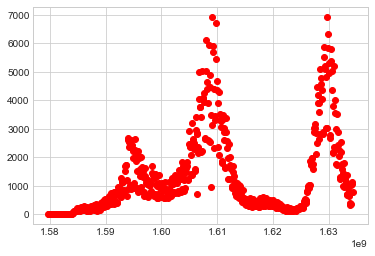
\includegraphics[scale=0.6]{Latext-Template/alabama_cases_dataset.png}
    \caption{Alabama's daily new case trend graph}
    \label{fig:input_dataset}
\end{figure}

In terms of data cleanliness, we haven't experienced any gaps in the CDC's trend data and the only conversion required is the aforementioned date to timestamp formatting step. It is important to reverse the order of the input data points due to the fast that when loading a CSV, the data point at index zero is actually the most recent case measurement, not the least recent. Other than this, the charts we found are very well formatted and consistent and require minimal preprocessing.

\subsection{Machine Learning Algorithms}
For this problem are using the multi-layer perceptron classifier provided by the sklearn.neural\_network.MLPClassifier package. Our algorithm consumes a range of trend data for COVID-19 cases in a given region and outputs future predicted trend data for a given number of days. For this problem, a neural network is appropriate because of the fast classification time and the ability for hidden layers to recognize subtle trend behaviors that would otherwise go unnoticed by other, less complex algorithms. For our initial attempt at using a neural network to solve this problem, we chose to use two hidden layers (sizes of 20 and then 4) as this gave the best results on our small training data set. We used the 'identity' activation function because our network needs to be able to output expected COVID-19 case numbers (which could number in the thousands) and other activation functions are limited to a maximum of one.

\begin{figure}
    \centering
    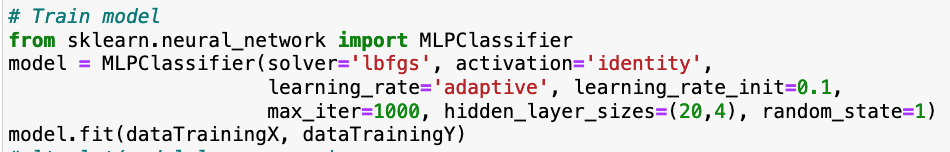
\includegraphics[scale=0.5]{Latext-Template/code.png}
    \caption{MLPClassifier parameters}
    \label{fig:MLPClassifier_code}
\end{figure}

\subsection{Implementation Details}
For testing and evaluating our initial approaches to this problem, we divided the Alabama trend data into training and test datasets split at a 7:3 ratio. This ratio was chosen because it separates a wide range of trend features into the training dataset, which is beneficial to the training process. We tried many different hidden layer values and ultimately arrived at our solution to this early implementation because it was the best choice that allowed the network to properly converge and still achieved somewhat reasonable accuracy on the test dataset.

\section{Comparison}
For our initial approach we tried a number of different training algorithms and network structures. As mentioned above, the first notable development was the conversion to the 'identity' activation function so that the network could produce output values in the ranges required for this problem. We tried solutions with no hidden layers and solutions with many staggered hidden layers and determined that the best test results were achieved with a structure somewhere between the two. We also determined that the best solver for this model was the 'lbfgs' algorithm, and despite a warning that the model failed to converge from the solver, our model was observed to converge nicely on the given training data (\ref{fig:training_accuracy}). The model still has trouble with certain sections of the test dataset (\ref{fig:test_accuracy}), however these can likely be fixed by increasing input data dimensionality and quantity.

\begin{figure}
    \centering
    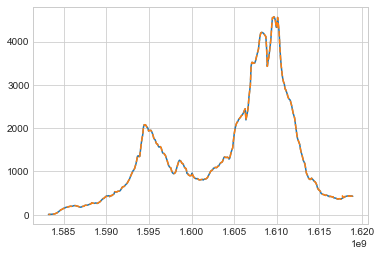
\includegraphics[scale=0.6]{Latext-Template/alabama_training.png}
    \caption{Training dataset performance (solid line = actual trend, dotted line = model's predicted trend, given the data for the previous 40 days)}
    \label{fig:training_accuracy}
\end{figure}

\begin{figure}
    \centering
    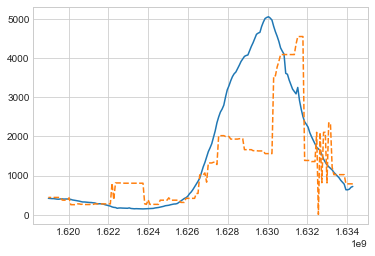
\includegraphics[scale=0.6]{Latext-Template/alabama_test.png}
    \caption{Test dataset performance (solid line = actual trend, dotted line = model's predicted trend, given the data for the previous 40 days)}
    \label{fig:test_accuracy}
\end{figure}

Comparing the results to existing solutions: random forest classifier, extra tree classifier (ETC), and support vector machine models. The random forest has an accuracy of more than 90 percent and the extra tree classifier has a 93.62 percent accuracy [3]. For the support vector machine models, the test accuracy of the joint, non-invasive, and invasive models were 0.80 ± 0.03, 0.77 ± 0.04, and 0.75 ± 0.4, respectively [4]. In general, all of these algorithms and models produce a relatively reasonable accuracy. However, the extra tree classifier is most accurate most likely because it is robust to outliers and has a lower risk of overfitting. Using COVID-19 data as the input, both of these attributes can have a huge impact.

\section{Future Directions}
In the future, we could parse other COVID-19 related data such as the demographics of individuals who have been diagnosed with COVID-19 and/or who have died from COVID-19 complications. With this information, we can predict how likely a person is of a certain demographic to be directly effected by the COVID-19 virus utilizing the same methodology and algorithms previously described. This data insight could be useful for doctors to make decisions on vaccination and treatment priority. Additionally, if time allowed, the RandomForestClassifier from sklearn.ensemble [6] could potentially be a better algorithm to use in addition to the artificial neural network based on its overall accuracy results compared to similar datasets and solved problems. 

\section{Conclusion}
In conclusion, the current implementation of the machine learning algorithms to predict COVID-19 data is insufficient and will need to vastly improved. Our plan to increase accuracy is to adjust the parameters of the algorithms currently in use such as the number of hidden layers, increase training data, and try various solver methods. Adjusting any of these will have a drastic impact on the accuracy and we can fine-tune our algorithm accordingly. Additionally, cleaning up noisy data will have a positive impact on the predicted results.

\bibliographystyle{IEEEtran}
\bibliography{}

[1] \emph{sklearn.neural\_network.MLPClassifier}, Accessed on: Nov. 8th, 2021 [Online]. Available: https://scikit-learn.org/stable/modules/generated/sklearn.neural\_network.MLPClassifier.html 

[2] Géron, A. (2019). \emph{Hands-on machine learning with Scikit-Learn, Keras, and TensorFlow : concepts, tools, and techniques to build intelligent systems.} Sebastopol, CA: O'Reilly Media, Inc.

[3] D. Painuli, D. Mishra, S. Bhardwaj, and M. Aggarwal, "Forecast and prediction of COVID-19 using machine learning," \emph{Data Science For COVID-19}, pp. 381-397, May 2021. 

[4] M. Mahdavi, H. Choubdar, E. Zabeh, M. Rieder, et al., "A machine learning based exploration of COVID-19 mortality risk", \emph{PLoS ONE}, July 2021. 

[5] \emph{sklearn.preprocessing.StandardScaler}, Accessed on: Nov. 8th, 2021 [Online]. Available: https://scikit-learn.org/stable/modules/generated/sklearn.preprocessing.StandardScaler.html

[6] \emph{sklearn.ensemble.RandomForestClassifier}, Accessed on: Nov. 8th, 2021 [Online]. Available: https://scikit-learn.org/stable/modules/generated/sklearn.ensemble.RandomForestClassifier.html 

\end{document}


